\documentclass[tikz,border=2pt]{standalone}
\usepackage{amsmath}
\usepackage{pgfplots}
\pgfplotsset{compat=1.18}

\begin{document}
% f(x)=x^3-3x: a local maximum at x=-1 and a local minimum at x=1. Each is the largest /
% smallest value only within a small neighbourhood (shaded) of the point, not on the whole domain.
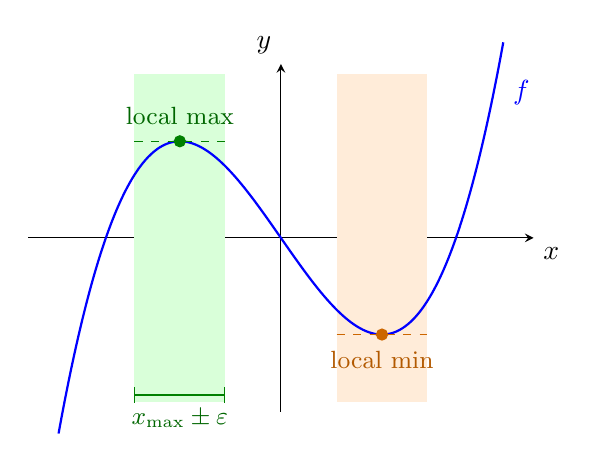
\begin{tikzpicture}
	\begin{axis}[
		axis lines=middle,
		xmin=-2.5, xmax=2.5,
		ymin=-3.6, ymax=3.6,
		xtick={-1,1}, xticklabels={$x_{\max}$,$x_{\min}$},
		ytick=\empty,
		xlabel={$x$}, ylabel={$y$},
		xlabel style={below right}, ylabel style={above left},
		samples=150, smooth, clip=false,
		width=8cm, height=6cm
		]
		\fill[green!15] (axis cs:-1.45,-3.4) rectangle (axis cs:-0.55,3.4);
		\fill[orange!15] (axis cs:0.55,-3.4) rectangle (axis cs:1.45,3.4);
		\addplot[thick, blue, domain=-2.2:2.2] {x^3-3*x};
		\addplot[only marks, mark=*, green!50!black] coordinates {(-1,2)};
		\addplot[only marks, mark=*, orange!80!black] coordinates {(1,-2)};
		\draw[dashed, green!50!black] (axis cs:-1.45,2) -- (axis cs:-0.55,2);
		\draw[dashed, orange!80!black] (axis cs:0.55,-2) -- (axis cs:1.45,-2);
		\node[green!40!black, anchor=south, font=\small] at (axis cs:-1,2.15) {local max};
		\node[orange!70!black, anchor=north, font=\small] at (axis cs:1,-2.15) {local min};
		\draw[green!50!black, |-|] (axis cs:-1.45,-3.25) -- (axis cs:-0.55,-3.25);
		\node[green!40!black, anchor=north, font=\small] at (axis cs:-1,-3.35) {$x_{\max}\pm\varepsilon$};
		\node[blue, anchor=west] at (axis cs:2.2,3.0) {$f$};
	\end{axis}
\end{tikzpicture}
\end{document}
